% ======================================================================
% TRB Annual Meeting Paper (unofficial) -- Research Manuscript
% Filled from the user-provided TRB 2027 template.
% ======================================================================

\documentclass[numbered]{trbunofficial}

% Supplemental packages needed by this manuscript; the template class
% supplies geometry, Times-like fonts, line numbering, captions, natbib,
% hyperlinks, headings, lists, equations, and title-page machinery.
\usepackage{booktabs}
\usepackage{tabularx}
\usepackage{array}
\usepackage{multirow}
\usepackage{makecell}
\usepackage{placeins}
\graphicspath{{../figures/}{figures/}{trb/figures/}}

\setlength{\emergencystretch}{2em}
\setlength{\textfloatsep}{9pt plus 2pt minus 2pt}
\setlength{\floatsep}{8pt plus 2pt minus 2pt}
\setlength{\intextsep}{8pt plus 2pt minus 2pt}
\newcolumntype{Y}{>{\raggedright\arraybackslash}X}
\newcolumntype{P}[1]{>{\raggedright\arraybackslash}p{#1}}
\newcommand{\ConVAE}{contrastive VAE}
\newcommand{\NCVAE}{noncontrastive VAE}
\newcommand{\TV}{\mathrm{TV}}

\begin{document}

% ---------- Title Page ----------
\title{When Survey Fidelity Is Not Traffic Validity: A Falsification-First Evaluation of Contrastive Trip Synthesis}

\TRBauthor*{Raziq Zaman}{Department of Civil and Environmental Engineering, University of Maryland}{raziq@umd.edu}[College Park, Maryland 20742, USA][0000-XXXX-XXXX-0001]
\TRBauthor{Raas Sarker Tomal}{Department of Civil and Environmental Engineering, University of Maryland}{rtomal@umd.edu}[College Park, Maryland 20742, USA][0000-XXXX-XXXX-0002]
\TRBauthor{Md Mahmudul Huque Chayan}{Department of Civil and Environmental Engineering, University of Maryland}{mchayan@umd.edu}[College Park, Maryland 20742, USA][0000-XXXX-XXXX-0003]
\TRBauthor{Darshan Pandit}{Department of Civil and Environmental Engineering, University of Maryland}{dmpandit@umd.edu}[College Park, Maryland 20742, USA][0000-XXXX-XXXX-0004]
\TRBauthor{Cinzia Cirillo}{Department of Civil and Environmental Engineering, University of Maryland}{ccirillo@umd.edu}[College Park, Maryland 20742, USA][0000-XXXX-XXXX-0005]

\AuthorHeaders{Zaman, Tomal, Chayan, Pandit, and Cirillo}

\TRBtitlefootnote{%
  This \LaTeX\ template is unofficial and may not meet current TRB requirements. Please review the latest submission rules at \href{https://trb.secure-platform.com/a/page/TRBPaperReview}{TRB’s Instructions for Authors} and ensure the paper is compliant. Noncompliant papers may be rejected. Template source: \url{https://github.com/chiehrosswang/TRB_LaTeX_tex}.
}

\maketitle

% ---------- Abstract ----------
\section{Abstract}
\noindent\textbf{Objectives:}~This study asks whether a deep generator that better preserves selected relationships in a weighted household travel survey also produces more credible transportation evidence outside that survey. It evaluates the proposition that trip synthesis should be qualified simultaneously for distributional fidelity, non-copying and support expansion, and operational traffic plausibility.

\hfill\break%
\noindent\textbf{Methods:}~A mixed-tabular variational autoencoder (VAE) synthesized 44 attributes from 110,926 weekday vehicle-trip records. A controlled contrastive regularizer preserved origin--destination (OD) and temporal fields in positive views while corrupting non-key attributes in negative views. One million records were generated by weighted bootstrap, a dependence-tree Bayesian network, a noncontrastive VAE, and the otherwise identical contrastive VAE. Internal tests covered marginals, nine prespecified cross-tabulations, exact matches, and row-level unseen-OD incidence. Independent roadway diagnostics projected straight tract-representative-point segments across 3,107 station-mapped boundaries and compared annual weekday counts and date-pooled hourly profiles.

\hfill\break%
\noindent\textbf{Findings:}~Relative to its VAE ablation, contrastive training reduced selected cross-table total variation by 11.4\% (seven of nine tables; paired Wilcoxon $p=0.027$) and unweighted numeric Kolmogorov--Smirnov distance by 12.5\%, while categorical total variation worsened 4.9\%. Both VAEs placed about 68.5\% of generated rows on OD pairs unseen in the survey and produced no exact 44-field matches under the implemented test. Yet bootstrap and the Bayesian network retained better overall survey fidelity. External evidence also changed the ranking: after date pooling removed a severe count-quantization artifact, the contrastive VAE improved normalized 24-hour profile error 21.1\% over its ablation, but the Bayesian network remained best and all methods had large volume bias.

\hfill\break%
\noindent\textbf{Novelty:}~The contribution is a falsification-first, same-support evaluation that connects a controlled trip-row contrastive ablation to independent annual and hourly roadside-count diagnostics and reports when internal and operational rankings diverge.

\hfill\break%
\noindent\textbf{Practical Applications:}~Agencies can use the proposed gates to reject generators that look statistically convincing but are too sparse, copied, geographically unconstrained, or volume-miscalibrated for demand-model inputs.

\newpage

\section{Introduction}

Household travel surveys are indispensable for observing activities, traveler attributes, modes, locations, and trip timing together. They are also sparse samples of a much larger combinatorial space. Classical population synthesis expands those samples using reweighting, simulation, graphical models, and control totals \cite{beckman1996creating,farooq2013simulation,sun2015bayesian}. Deep generative models promise a different advantage: they can learn high-dimensional nonlinear associations and generate records beyond the exact support of the survey \cite{borysov2019microagents,garrido2020rare,kim2023feasible}. For trip synthesis, however, additional rows are useful only if they retain behavioral structure and remain credible when exposed to transportation evidence not used during training.

Most synthetic-mobility evaluations emphasize internal evidence: marginal distances, pairwise associations, sequence similarity, feasibility rules, diversity, or disclosure proxies \cite{kapp2024review,choi2025tutorial,wu2026evaluation}. Those tests are necessary but not sufficient. A generator can preserve one-dimensional histograms while breaking mode--time or distance--duration dependence. It can avoid exact copies by emitting improbable combinations. It can also expand OD support yet fail to reproduce traffic volumes or temporal profiles. Conversely, an exact weighted resample can achieve near-perfect survey fidelity by copying source records. These are not variations of a single objective; they are competing qualifications.

External validation has precedents. Generative activity models have been compared with ground-truth activities and traffic simulation \cite{yin2018activities}; recent mobility models have used observed traffic or cellular signaling outside the training source \cite{ma2025foundation,vo2026harnessing}. The unresolved operational question is narrower: when a controlled change improves a trip generator's internal dependence metrics, does that ranking persist under identical-support roadside-count diagnostics? This study uses annual and hourly count sources as deliberate stress tests, not as training targets and not as a substitute for network assignment.

We examine three research questions:

\begin{enumerate}[leftmargin=0.27in,itemsep=1pt,topsep=3pt]
\item Does trip-specific contrastive regularization improve selected numeric and cross-attribute relationships relative to an otherwise identical mixed-tabular VAE?
\item What trade-off emerges among survey fidelity, exact copying, and generation on OD pairs unseen in the survey?
\item Do internal rankings survive an audited, common-support comparison with independent annual weekday counts and date-pooled hourly traffic profiles?
\end{enumerate}

The paper makes three contributions. First, it specifies a survey-weight-aware mixed-tabular VAE with a controlled binary contrastive encoder regularizer and a zero-coefficient ablation. Second, it evaluates four generators through separate fidelity, dependence, copying, and unseen-support lenses rather than collapsing them into one score. Third, it develops and audits a two-timescale roadside-count diagnostic. The audit is consequential: an apparently large hourly improvement in the archived exact-date analysis disappears after correcting method-specific temporal expansion and sparse one-event count quanta. The remaining result is more useful: contrastive learning improves hourly \emph{shape} relative to the matched VAE, but neither deep model is best on absolute external traffic evidence. Figure~\ref{fig:workflow} summarizes this falsification-first logic.

\begin{figure}[!htbp]
\centering
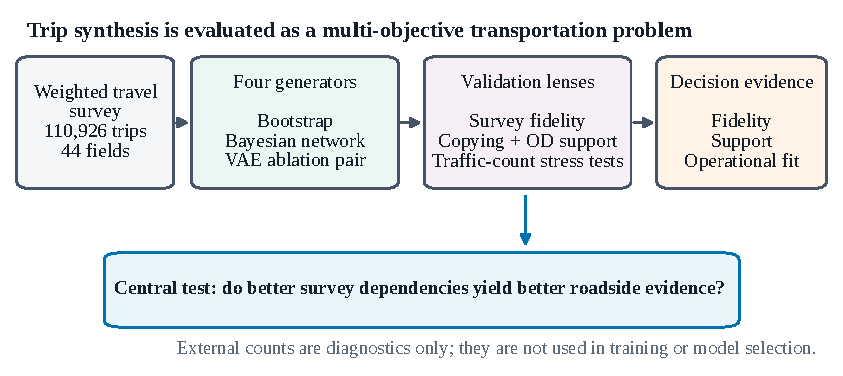
\includegraphics[width=\textwidth]{fig_01_workflow.pdf}
\caption{Research design. Survey similarity, non-copying and support, and independent traffic evidence are treated as distinct validation lenses. External counts are untouched diagnostics rather than loss terms or model-selection targets.}
\label{fig:workflow}
\end{figure}

\section{Deep Generative Trip Synthesis and the Validation Gap}

\subsection{From population controls to deep joint distributions}

Traditional synthetic-population methods reconstruct agents compatible with microdata and aggregate controls. Reweighting and combinatorial procedures established the baseline problem \cite{beckman1996creating}; simulation-based optimization, Bayesian networks, and hidden Markov formulations expanded the available dependence structures \cite{farooq2013simulation,sun2015bayesian,saadi2016hidden}. Open-data workflows now connect synthetic populations to full travel-demand inputs \cite{horl2021paris}. These methods retain a transportation advantage: their constraints, conditional structure, and control totals are explicit.

Deep population synthesis trades some of that transparency for flexible representation learning. Variational autoencoders (VAEs) \cite{kingma2014vae} and generative adversarial networks for tabular data \cite{xu2019ctgan} have been adapted to micro-agent generation, rare combinations, household--person consistency, and feasibility \cite{borysov2019microagents,garrido2020rare,aemmer2022joint,kim2023feasible}. The central methodological challenge is mixed data: high-cardinality geography, nominal choices, ordered counts, continuous distance, and survey expansion weights must coexist in one record.

\subsection{Trips, activities, schedules, and trajectories}

The output unit matters. Population synthesis generates people or households; trip-row synthesis generates a multivariate trip record; schedule synthesis generates ordered activity episodes; trajectory synthesis generates spatial sequences. Bayesian activity generation \cite{joubert2020bayesian}, composite travel GANs \cite{badumarfo2022composite}, conditional smart-card imputation \cite{kim2022tripchains}, and synthetic smart-card trips \cite{kieu2023smartcard} show that tabular and sequential outputs require different coherence tests. Urban mobility VAEs and imitation-learning trajectory generators add spatial sequence structure \cite{huang2019urbanvae,choi2021trajgail}. More recent work fuses surveys with smart cards, generates full schedules, and learns broad mobility representations \cite{lee2025collagan,shone2025scheduling,ma2025foundation,liao2026deepactivity,lu2026pop2actloc}.

Contrastive representation learning encourages related views to be nearby and corrupted views to be separated \cite{oord2018cpc}. In tabular data, random feature corruption can produce useful self-supervision \cite{bahri2022scarf}. Transportation records require domain-aware views: changing destination, day, or departure time can change the trip itself, whereas light corruption of a non-key household or vehicle field can preserve the trip's spatiotemporal identity. The present experiment therefore protects OD and time in its positive view and uses a same-architecture, same-seed zero-contrastive ablation to isolate the incremental effect.

\begin{table}[!htbp]
\caption{Literature streams and the specific validation gap addressed here.}
\label{tab:literature}
\centering
\setlength{\tabcolsep}{4pt}
\begin{tabularx}{\textwidth}{P{0.20\textwidth}Y Y}
\toprule
\textbf{Stream} & \textbf{Representative contribution} & \textbf{Implication for this study} \\
\midrule
Controlled population synthesis & Reweighting, simulation, graphical models, and public-data demand systems \cite{beckman1996creating,farooq2013simulation,sun2015bayesian,horl2021paris} & Preserve explicit controls and baselines; a deep generator must beat more than an unweighted sample. \\
Deep population synthesis & Nonlinear joint distributions, rare combinations, joint household--person attributes, and feasibility \cite{borysov2019microagents,garrido2020rare,aemmer2022joint,kim2023feasible} & Evaluate dependence and feasible support separately from marginal fit. \\
Trip and schedule synthesis & Tabular/sequential travel records, smart-card imputation, and multimodal activity schedules \cite{badumarfo2022composite,kim2022tripchains,kieu2023smartcard,lee2025collagan,shone2025scheduling} & Match the metric to the generated unit; this paper evaluates trip rows, not full tours. \\
External mobility validation & Ground-truth activities, traffic simulation or observations, and cellular signaling \cite{yin2018activities,ma2025foundation,vo2026harnessing} & External validation is not new; identical support and diagnostic scaling are the unresolved focus. \\
Evaluation and disclosure & Reviews and representativeness--privacy--utility frameworks \cite{kapp2024review,choi2025tutorial,wu2026evaluation,stadler2022groundhog} & No exact copies is a diagnostic, not a formal privacy guarantee. \\
\bottomrule
\end{tabularx}
\end{table}

The literature thus does not support a claim of first external validation. It supports a more precise gap. Same-architecture trip-row ablations are rarely carried from weighted survey metrics to untouched, two-timescale roadside evidence on identical evaluation support. The field also risks equating favorable internal rankings with operational validity and absence of exact matches with privacy. This paper is designed to test, and potentially falsify, both inferences.

\section{Data and Experimental Design}

\subsection{Travel-survey table}

The transformed input combines the 2018--2019 Maryland Statewide Household Travel Survey and the 2017--2018 Metropolitan Washington Council of Governments Regional Travel Survey \cite{bmc2020mts,mwcog2019rts}. The archived model table contains 110,926 weekday vehicle-trip rows, 44 synthesized fields, and one excluded expansion-weight field. Dates span October 10, 2017, through July 11, 2019, with 423 observed departure dates and day-of-week categories Monday through Friday.

The 44 fields comprise 26 categoricals, 17 ordinal integers, and one continuous field. They cover origin and destination activity and census tract; mode, parking, occupancy, toll and vehicle attributes; departure time, reported time, and distance; home and work geography; and household/person attributes. Missing values had been filled before the frozen experiment. Reported travel time and distance use $-1$ sentinels for some missing values, which the model treats as numeric values. The retained source field is the household final weight, renamed \texttt{weight}; its sum over trip rows is 19,287,211.907. We call this the \emph{weighted trip expansion total}, not a population estimate. Its use at trip-row level must be interpreted as the repository's weighting design and is revisited under limitations.

The VAE split was 88,741 training and 22,185 validation rows. Its preprocessor was fitted only on training rows. The weighted bootstrap and Bayesian network were fitted to all 110,926 rows, giving those baselines more source information. All internal metrics compare generated data with the full transformed table; they are therefore model-reproduction diagnostics, not held-out downstream utility tests.

\subsection{Generators and frozen run}

Four methods generated at most 1,000,000 records each under seed 20260611:

\begin{enumerate}[leftmargin=0.27in,itemsep=1pt,topsep=3pt]
\item \textbf{Weighted bootstrap:} sample rows with replacement in proportion to the retained expansion field.
\item \textbf{Bayesian network:} fit a Chow--Liu dependence tree \cite{chow1968dependence}, discretizing numeric variables into at most 16 bins with additive smoothing 1.0.
\item \textbf{Noncontrastive VAE:} fit the mixed-tabular VAE with contrastive coefficient zero.
\item \textbf{Contrastive VAE:} fit the identical architecture and seed with contrastive coefficient 0.25.
\end{enumerate}

The 19.287-million weighted total was represented by one million sampled rows; count diagnostics multiply raw crossing events by a common sample factor 19.287212. This cap is adequate for internal distributions but, as the independent count stress tests show, can be too coarse for exact screenline-date-hour cells.

\subsection{Independent geographic and count data}

Census 2019 TIGER/Line tracts provide geometry \cite{census2019tiger}. Filtering Maryland, the District of Columbia, and Virginia to tract codes present in the survey leaves 2,232 tracts. Their adjacencies yield 3,257 candidate tract-boundary screenlines; 3,107 have at least one mapped Maryland Department of Transportation State Highway Administration station. The dense external target is the 2018 annual average weekday traffic field \texttt{AAWDT\_2018} \cite{mdot2018aawdt}. The sparse temporal target is Federal Highway Administration Traffic Monitoring Analysis System hourly station data \cite{fhwa2018tmas,fhwa2022tmg}: 64 stations, 37,800 station-days, and 907,200 station-hours in the downloaded source, of which 37 stations map to 56 hourly screenlines.

Neither source enters training, checkpoint selection, or hyperparameter selection. They are diagnostic proxies. Multiple screenlines can reuse a station, and hourly station counts are scaled by that station's annual share of its mapped screenline. Results therefore use screenline-block resampling and are not interpreted as independent traffic assignment observations.

\section{Methods}

\subsection{Mixed-tabular variational autoencoder}

Each categorical field is integer encoded and embedded; the 26 embedding blocks contribute 262 values. The 18 numeric fields are standardized and concatenated, producing 280 inputs. A four-layer encoder with widths 512, 499, 487, and 475, LayerNorm, rectified-linear activations, and dropout 0.02 maps each record to 512-dimensional Gaussian mean and log-variance vectors. A mirrored decoder produces 26 categorical softmax heads and 18 numeric outputs. The model has 8,302,216 trainable parameters.

Let $x_i=(x_i^{c},x_i^{n})$ denote the categorical and numeric components, and let $w_i$ be its transformed survey weight. The row reconstruction term sums categorical cross-entropies and numeric squared errors; reconstruction and Kullback--Leibler (KL) terms are averaged with $w_i$. Training weights are capped at the training-set 99th percentile (671.73) and normalized to mean one. This clips 905 training rows and about 1.16\% of raw training weight mass. The objective is

\begin{linenomath*}
\begin{equation}
\mathcal{L}=\mathcal{L}_{\mathrm{rec},w}+0.03\,\mathcal{L}_{\mathrm{KL},w}+\lambda\,\mathcal{L}_{\mathrm{con}},
\label{eq:loss}
\end{equation}
\end{linenomath*}
where $\lambda=0$ for the noncontrastive VAE and 0.25 for the contrastive VAE. AdamW uses learning rate $5\times10^{-4}$, batch size 2,048, gradient clipping 5, and at most 1,260 epochs. Validation checkpointing minimizes weighted reconstruction plus KL, excluding the contrastive term. The selected epochs are 195 and 196 for the noncontrastive and contrastive models, respectively.

Sampling draws $z\sim\mathcal{N}(0,I)$. Categorical logits are divided by temperature 0.75 and multinomially sampled. Numeric outputs are inverse transformed; ordinal fields are rounded and all numerics are clipped to training ranges. The weight is never generated. Consequently, valid categorical labels and in-range numbers are partly guaranteed by decoding and postprocessing and are not treated as independent evidence of quality.

\subsection{Trip-specific binary contrastive regularization}

For an anchor record, the positive view protects origin tract, destination tract, survey week, day of week, and departure time. Other categorical fields are independently replaced with probability 0.03; other standardized numerics receive Gaussian jitter with standard deviation 0.02. The negative view draws each categorical code uniformly from its vocabulary and shuffles each numeric column within the batch. Despite the archived configuration label \texttt{marginal}, categorical negatives are uniform rather than empirical-marginal draws.

The encoder means for anchor, positive, and negative records are unit-normalized. Their cosine similarities form a two-logit cross-entropy at temperature 0.10, with the positive as the target. This is a binary contrastive regularizer, not the conventional many-negative InfoNCE objective. High-cardinality uniform geographic draws may also make negatives unusually easy. The controlled ablation isolates the observed effect of this implementation, rather than claiming a universally optimal contrastive design. Figure~\ref{fig:architecture} gives the complete data flow.

\begin{figure}[!htbp]
\centering
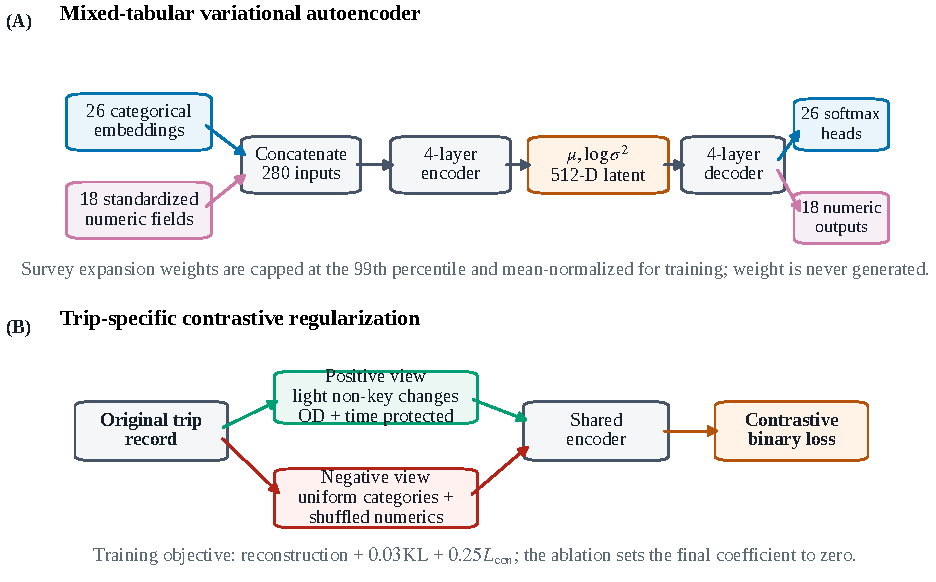
\includegraphics[width=\textwidth]{fig_02_architecture.pdf}
\caption{Model and contrastive ablation. (A) Mixed categorical embeddings and standardized numerics enter a four-layer VAE. (B) Positive views preserve trip-defining OD and time fields; negative views use uniform categorical draws and within-batch numeric shuffles. The noncontrastive ablation sets only $\lambda$ in Equation~\ref{eq:loss} to zero.}
\label{fig:architecture}
\end{figure}

\begin{table}[!htbp]
\caption{Frozen experimental configuration required for reproduction.}
\label{tab:config}
\centering
\footnotesize
\setlength{\tabcolsep}{4pt}
\begin{tabularx}{\textwidth}{P{0.21\textwidth}Y P{0.21\textwidth}Y}
\toprule
\textbf{Component} & \textbf{Setting} & \textbf{Component} & \textbf{Setting} \\
\midrule
Input & 110,926 rows; 44 fields & Output cap & 1,000,000 per method \\
VAE split & 80/20; seed 20260611 & Latent/input & 512/280 \\
Hidden widths & 512, 499, 487, 475 & Optimization & AdamW; $5\times10^{-4}$; batch 2,048 \\
Epoch budget & 1,260; best checkpoint & Dropout/normalization & 0.02/LayerNorm \\
KL coefficient & 0.03 & Contrast coefficient & 0 or 0.25 \\
Contrast temperature & 0.10 & Sampling temperature & 0.75 \\
Positive corruption & 0.03 categorical; 0.02 numeric & Protected fields & OD, week, weekday, departure time \\
Negative corruption & uniform categorical; shuffled numeric & Weight transform & cap at q99; normalize mean to one \\
\bottomrule
\end{tabularx}
\end{table}

\subsection{Screenline projection and temporal aggregation}

A synthetic OD path is the straight segment between tract representative points. Every intersected tract boundary is a candidate crossing; it is not a routed road path. A count station belongs to a boundary when its boundary distance is less than half its distance to the nearest tract representative point. Crossing time is departure time plus reported travel time multiplied by the boundary's ordered fraction along the segment. For multiple crossings, fraction $j/(J+1)$ is used for crossing $j$ of $J$.

Annual synthetic crossings are expanded by the 19.287212 sample factor and divided by each method's reconstructed departure-date count: 423 for bootstrap, 452 for the Bayesian network and noncontrastive VAE, and 453 for the contrastive VAE. The observed field is explicitly interpreted as annual average weekday traffic. Because all source and generated day-of-week categories are Monday through Friday, relabeling the archived \texttt{average\_day} calculation as average weekday changes no value.

Exact-date hourly comparison is inappropriate for the capped samples. In the archive, a single event became 8,486--9,856 vehicles after multiplication by both the sample factor and a method-specific temporal factor. Synthetic zero shares reached 91.1--99.1\%, although observed proxy zeros were 0.014\%. We therefore pool weekday crossing dates before comparison. For method $m$, screenline $s$, and hour $h$,

\begin{linenomath*}
\begin{equation}
S_{msh}=\sum_{d\in\mathrm{weekdays}}
\frac{\widetilde{S}_{msdh}}{F_m},
\qquad
\TV_{ms}=\frac{1}{2}\sum_{h=0}^{23}
\left|\frac{S_{msh}}{\sum_h S_{msh}}-
\frac{O_{sh}}{\sum_h O_{sh}}\right|,
\label{eq:hourly}
\end{equation}
\end{linenomath*}
where $\widetilde{S}$ is the stored expanded count, $F_m$ is its temporal expansion factor, and $O_{sh}$ averages all available observed weekdays. Pooling retains the common sample factor and reduces the smallest positive increment to 19.287 vehicles. All methods are evaluated on the identical $56\times24=1,344$ screenline-hour grid; absent synthetic cells are zeros. A screenline with no crossings receives profile TV 1. Figure~\ref{fig:screenline} illustrates the diagnostic.

\begin{figure}[!htbp]
\centering
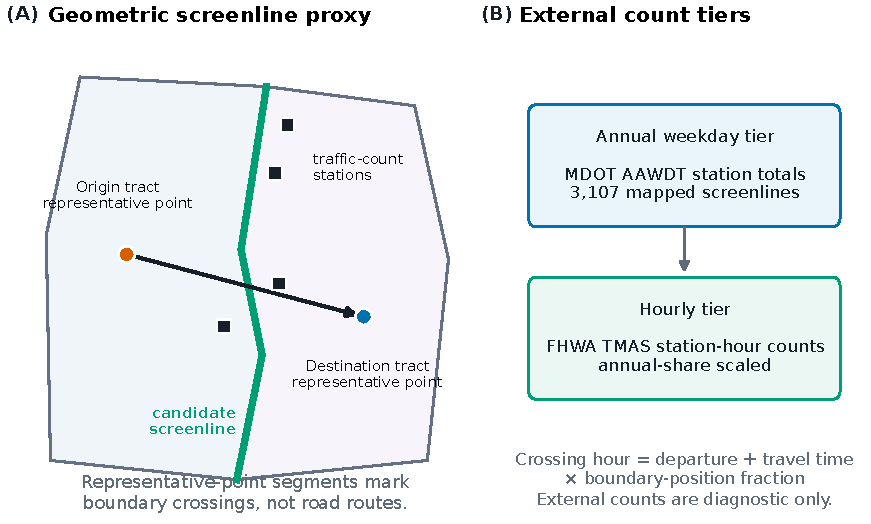
\includegraphics[width=\textwidth]{fig_04_screenline_method.pdf}
\caption{External diagnostic construction. Straight tract-representative-point segments indicate geometric boundary crossings, not assigned road routes. Annual station totals provide a dense spatial stress test; hourly station profiles provide a sparse temporal stress test after scaling by annual station share.}
\label{fig:screenline}
\end{figure}

\section{Evaluation}

\subsection{Internal fidelity and dependence}

Categorical fidelity uses weighted total variation (TV) between survey and synthetic proportions. Numeric fidelity uses the two-sample Kolmogorov--Smirnov (KS) statistic. In the frozen implementation, KS and Wasserstein calculations are unweighted even though numeric mean and standard-deviation summaries use survey weights; results are labeled accordingly. Dependence fidelity uses TV for nine prespecified cross-tabulations: activity--mode, mode--departure bin, origin county--destination county, distance bin--travel-time bin, household income--mode, employment--mode, household size--vehicle count, vehicle model year--vehicle, and age--license.

The contrastive and noncontrastive VAEs are paired across 26 categorical fields, 18 numeric fields, and nine cross-tables. Two-sided Wilcoxon signed-rank tests assess whether feature-level differences are centered at zero \cite{wilcoxon1945rank}. With only nine cross-tables, the test is interpreted with its effect direction and count of improved tables, not as a standalone discovery claim.

\subsection{Copying and unseen OD support}

Exact-row copying is the fraction of generated records exactly matching any source row across all 44 synthesized fields. The duplicate rate is the share of generated records duplicated within the sample. Row-level unseen-OD share is the fraction of generated \emph{rows} whose directed tract pair did not occur in the source survey. It is not the share of unique OD pairs, and ``unseen'' does not imply feasible or behaviorally plausible. Exact equality across a continuous distance field is also a weak memorization test. These metrics are therefore non-copying and support diagnostics, not differential-privacy or membership-inference guarantees \cite{stadler2022groundhog}.

\subsection{External metrics and uncertainty}

Annual and date-pooled hourly absolute fit uses root mean square error (RMSE), mean absolute error (MAE), mean bias, and Pearson correlation after $\log(1+x)$ transformation. Temporal shape uses Equation~\ref{eq:hourly}. Confidence intervals use 10,000 paired percentile bootstrap replicates at the screenline level, retaining all 24 hours within a selected block \cite{efron1993bootstrap}. Pairing is essential because every method is evaluated on the same screenline grid. Intervals reflect geographic-block variation only; they do not include model-training or synthetic-draw uncertainty from the single seed.

\section{Results}

\subsection{Internal trade-offs}

Table~\ref{tab:internal} reports the frozen internal results. Weighted bootstrap nearly reproduces the survey by construction: mean categorical TV is 0.0033 and mean cross-table TV is 0.0050, but every output row is a source copy. The Bayesian network retains comparable one-dimensional fidelity and improves on exact copying, while its mean cross-TV rises to 0.0901. Both VAEs sacrifice more marginal and cross-table fidelity to generate beyond exact source records.

The controlled contrastive effect is directional rather than universal. Relative to the noncontrastive VAE, the contrastive VAE reduces mean unweighted numeric KS from 0.1261 to 0.1103 (12.5\%) and selected cross-TV from 0.2556 to 0.2265 (11.4\%). It improves seven of nine cross-tables; the paired cross-table test gives $p=0.027$. The numeric improvement occurs for 11 of 18 fields but is not significant as a paired field test ($p=0.304$). Mean categorical TV worsens from 0.0621 to 0.0652 (4.9\%; $p=0.408$), with improvement in only 12 of 26 fields. Absolute errors also remain high for difficult tables: vehicle-model-year by vehicle TV is 0.778 after contrastive training, and origin-county by destination-county TV is about 0.379.

\begin{table}[!htbp]
\caption{Internal survey reproduction, copying, and unseen-support results. Lower is better for TV and KS. Numeric KS is unweighted in the frozen implementation; categorical and cross-table survey proportions are weighted.}
\label{tab:internal}
\centering
\setlength{\tabcolsep}{3.4pt}
\begin{tabularx}{\textwidth}{Y r r r r r}
\toprule
\textbf{Method} & \textbf{Cat. TV} & \textbf{Num. KS} & \textbf{Cross TV} & \textbf{Exact copy} & \textbf{Unseen-OD row share} \\
\midrule
Weighted bootstrap & \textbf{0.0033} & 0.0439 & \textbf{0.0050} & 1.0000 & 0.0000 \\
Bayesian network & 0.0034 & \textbf{0.0437} & 0.0901 & 0 & 0.3330 \\
Noncontrastive VAE & 0.0621 & 0.1261 & 0.2556 & 0 & \textbf{0.6856} \\
Contrastive VAE & 0.0652 & 0.1103 & 0.2265 & 0 & 0.6852 \\
\bottomrule
\end{tabularx}
\end{table}

The copying--support lens changes the preference order. Both VAEs and the Bayesian network yield zero exact 44-field matches and zero within-sample duplicates; bootstrap has exact-copy rate 1.0 and duplicate rate 0.8918. The two VAEs place about 68.5\% of generated rows on directed OD pairs unseen in the source; the Bayesian network places 33.3\%. Those pairs are novel relative to the survey, not proven feasible. Figure~\ref{fig:tradeoff} makes the resulting frontier explicit: survey reproduction, non-copying, and broader support cannot be summarized honestly by a single leaderboard.

\begin{figure}[!htbp]
\centering
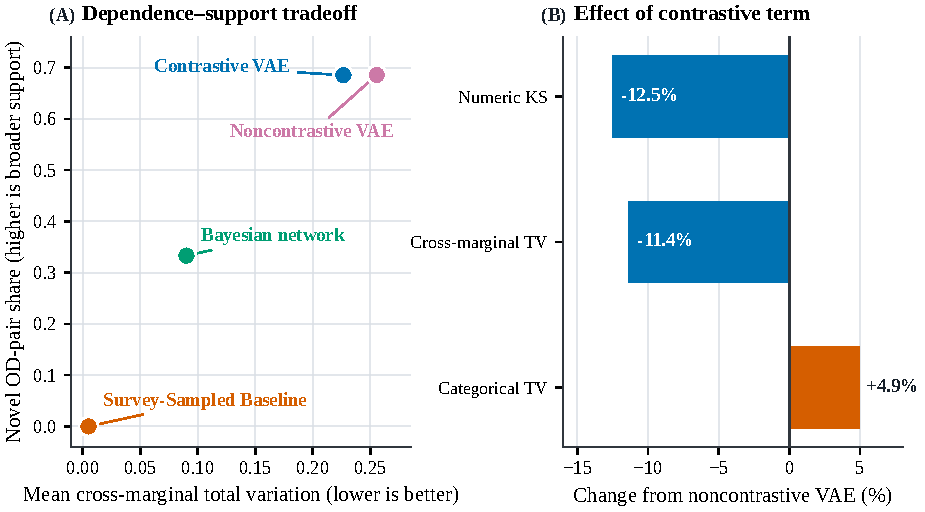
\includegraphics[width=\textwidth]{fig_03_internal_tradeoff.pdf}
\caption{Internal trade-offs. (A) Weighted bootstrap occupies the survey-fidelity corner by exact copying; learned methods generate more rows on unseen OD pairs at the cost of larger cross-table error. (B) The contrastive term improves numeric KS and selected cross-table TV but worsens categorical TV. Only the paired cross-table improvement is significant at 0.05.}
\label{fig:tradeoff}
\end{figure}

Training cost also rises. Archived runtimes are 6.84 seconds for bootstrap, 76.44 seconds for the Bayesian network, 537.87 seconds for the noncontrastive VAE, and 896.31 seconds for the contrastive VAE. Contrastive training is 66.6\% slower than its ablation. The best checkpoints occur near epoch 195, although training continues to epoch 1,260 and final validation loss deteriorates, suggesting that more aggressive early stopping would save computation without changing the selected artifacts.

\subsection{Independent count stress tests}
\label{sec:externalresults}

Annual average weekday results are uniformly weak (Table~\ref{tab:external}). The Bayesian network has the lowest RMSE, 55,772 vehicles, followed by the noncontrastive VAE (56,145), bootstrap (56,659), and contrastive VAE (57,843). Log correlations range only 0.169--0.217, and every method underpredicts on average. The contrastive VAE's mean bias is $-22,120$, worse than its ablation. These magnitudes do not validate any generator as a traffic-demand model.

The archived exact-date hourly leaderboard is more misleading. Its temporal expansion factors differ by method because crossing dates depend on generated travel time and post-midnight offsets. One crossing expands into 8,486--9,856 vehicles, making the median synthetic cell zero for every method and median absolute percentage error 100\%. An apparent roughly 51\% learned-model RMSE reduction relative to bootstrap is therefore a sparse-quantization effect and is not reported as a performance result.

Date pooling before undoing temporal expansion produces a defensible common $56\times24$ comparison. Absolute RMSE remains 5,916--6,193 vehicles, and every method retains mean underprediction exceeding 4,100 vehicles. The Bayesian network is best on RMSE and both raw and log correlation. Contrastive RMSE is 263 vehicles worse than noncontrastive (paired 95\% confidence interval 207--324). Thus the external absolute-volume ranking contradicts the internal contrastive dependence ranking.

A positive but bounded result remains for temporal shape. After normalizing each screenline to a 24-hour distribution, mean profile TV is 0.309 for bootstrap, 0.141 for the Bayesian network, 0.249 for the noncontrastive VAE, and 0.197 for the contrastive VAE. Contrastive training improves its matched ablation by 21.1\% (paired 95\% confidence interval 16.8--25.5\%), although the Bayesian network remains best. Figure~\ref{fig:hourly} shows both conclusions. Contrastive representation learning improves allocation of a miscalibrated volume across the day, but it does not solve external volume calibration.

\begin{table}[!htbp]
\caption{Independent roadway-count stress tests. Annual rows use 3,107 station-mapped screenlines. Hourly rows pool dates before temporal expansion and use 1,344 identical screenline-hour cells.}
\label{tab:external}
\centering
\setlength{\tabcolsep}{3.2pt}
\begin{tabularx}{\textwidth}{Y r r r r r}
\toprule
\textbf{Method} & \multicolumn{2}{c}{\textbf{Annual weekday}} & \multicolumn{3}{c}{\textbf{Date-pooled hourly}} \\
\cmidrule(lr){2-3}\cmidrule(lr){4-6}
 & \textbf{RMSE} & \textbf{Log $r$} & \textbf{RMSE} & \textbf{Log $r$} & \textbf{Profile TV} \\
\midrule
Weighted bootstrap & 56,659 & 0.215 & 6,086 & 0.610 & 0.309 \\
Bayesian network & \textbf{55,772} & \textbf{0.217} & \textbf{5,916} & \textbf{0.696} & \textbf{0.141} \\
Noncontrastive VAE & 56,145 & 0.169 & 5,929 & 0.659 & 0.249 \\
Contrastive VAE & 57,843 & 0.173 & 6,193 & 0.669 & 0.197 \\
\bottomrule
\end{tabularx}
\end{table}

\begin{figure}[!htbp]
\centering
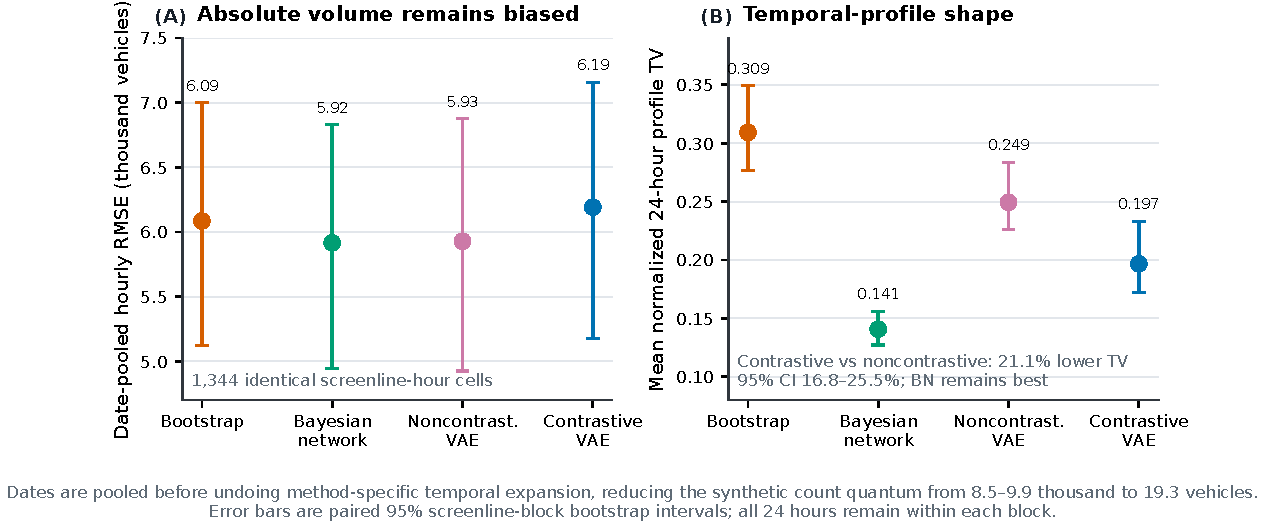
\includegraphics[width=\textwidth]{fig_05_hourly_granularity.pdf}
\caption{Audited hourly stress test. (A) Pooling dates before undoing temporal expansion removes the exact-date count quantum but leaves large absolute RMSE and overlapping block-bootstrap intervals. (B) The contrastive term improves normalized temporal profile TV relative to the matched VAE, but the Bayesian network remains best. Error bars are paired 95\% screenline-block bootstrap intervals.}
\label{fig:hourly}
\end{figure}

\FloatBarrier
\section{Discussion and Practical Applications}

\subsection{What is seminal for trip synthesis}

The most important result is not that one architecture wins. It is that a trip generator can improve a controlled internal dependence target, expand observed support, and still fail an external volume test. This separates three questions that are often conflated:

\begin{enumerate}[leftmargin=0.27in,itemsep=2pt,topsep=3pt]
\item \textbf{Can the model reproduce what the survey measured?} Bootstrap dominates because it copies; the Bayesian network provides a strong low-cost generative baseline.
\item \textbf{Can the model create records beyond exact survey rows?} Both VAEs and the Bayesian network do so under the implemented exact-match test, and the VAEs place many rows on unseen OD pairs.
\item \textbf{Can the output survive untouched transportation evidence?} None is volume-calibrated; contrastive training improves only the scale-free hourly shape relative to its ablation.
\end{enumerate}

This decomposition is consequential for model development. If the study had reported only marginal and cross-table averages, the contrastive VAE could be presented as a broad improvement over its ablation. If it had reported the archived exact-date count leaderboard, it could also appear to halve hourly RMSE. Auditing the count quantum, temporal denominator, and common support falsifies the second inference. The result illustrates why operational evaluation code deserves the same scrutiny as the generator.

Contrastive learning nevertheless contributes a useful mechanism. Protecting OD and time in positive views encourages an encoder that better retains selected joint structure and, externally, improves the normalized 24-hour profile. The gain is limited by its negatives: uniform draws over large tract vocabularies can be too easy and need not represent plausible alternatives. Hard negatives conditioned on geography, household constraints, land use, and network accessibility are a clear next step.

\subsection{An agency qualification workflow}

A practical deployment should use sequential gates rather than one composite score:

\begin{enumerate}[leftmargin=0.27in,itemsep=2pt,topsep=3pt]
\item \textbf{Schema gate:} verify valid categories, numeric bounds, missingness mechanisms, and immutable fields; distinguish properties enforced in postprocessing from learned properties.
\item \textbf{Survey gate:} report weighted marginals and prespecified behavioral crosses with feature-level distributions, not only averages.
\item \textbf{Non-copying/support gate:} report exact and near-neighbor disclosure diagnostics, within-sample duplicates, and unseen OD incidence; test structural feasibility before calling unseen pairs plausible.
\item \textbf{External gate:} freeze model selection, use untouched sources, force identical spatial and temporal support, and disclose every expansion denominator and prediction quantum.
\item \textbf{Assignment gate:} before forecasting, route trips on a network and calibrate aggregate demand separately from distributional generation.
\end{enumerate}

The generator and calibrator should remain conceptually distinct. Survey-weighted synthesis can propose a high-dimensional trip table; a network-aware model can then impose travel times, feasible OD paths, capacity, and traffic-count constraints. Count residuals should identify where the synthesis-to-assignment pipeline requires correction, not be hidden inside a global accuracy score.

\section{Limitations and Reproducibility}

The study is a single-seed experiment. Bootstrap intervals resample screenlines, not model training or synthetic draws. Repeated seeds and a nested model-selection holdout are required before generalizing small differences. Baselines use all source rows while the VAEs use an 80\% training split, favoring the baselines for survey reproduction. Numeric KS and Wasserstein metrics are unweighted in the frozen implementation, although categorical proportions, numeric mean/standard deviation, and VAE losses use weights.

The retained weight originated as a household final weight; the historical preprocessing discarded the trip-final weight. Applying household inclusion weights to trip rows can be defensible, but the survey data dictionaries and rationale must be verified before using the 19.287-million expansion total operationally. Missing time and distance sentinels are modeled as $-1$ without separate missingness indicators. The raw-to-model preprocessing scripts for intermediate stages are not all preserved on this branch.

Non-copying evidence is limited. Equality across all 44 fields, including continuous distance, can miss near copies; no nearest-neighbor, membership-inference, or differential-privacy analysis is enabled. Unseen OD pairs have not been checked against land use or road accessibility. The path cache also truncates candidate OD pairs at 250,000 after concatenating methods in fixed order, so earlier methods consume the cap and full support is not treated symmetrically.

External counts are proxies. Straight centroid-line crossings omit route choice and network topology. Annual station assignments reuse some stations across screenlines; the 56 hourly screenlines derive from only 37 stations. Hourly observations divide a station count by its annual screenline share. Date pooling fixes the documented expansion artifact but does not remove sample Monte Carlo error or absolute demand bias. These limitations explain why the count analysis is a stress test, not validation of a deployable assignment model.

The frozen run retains configuration snapshots, best VAE checkpoints, training histories, validation tables, geographic caches, and count comparisons at repository commit \texttt{95dab02c}. It does not retain one-million-row samples, the fitted baseline artifacts, the claimed hyperparameter-sweep results, a package lockfile, or complete hardware metadata. Accordingly, unsupported sweep and unique-OD-count claims are omitted. Code and archived artifacts are available at \url{https://github.com/RaziqZaman/tripsynth} on branch \texttt{wctr-aadt}; the figure script recomputes the corrected date-pooled analysis directly from preserved Parquet files.

\section{Conclusions}

A trip-synthesis model should be judged by more than closeness to its survey. In a controlled mixed-tabular VAE ablation, trip-specific contrastive training reduces selected cross-table TV 11.4\% and improves normalized external hourly profile TV 21.1\% relative to the same VAE without the term. Those gains coexist with worse categorical fidelity, higher runtime, inferior survey reproduction to simpler baselines, and no absolute traffic-volume advantage. Weighted bootstrap is faithful because it copies; the Bayesian network is the strongest overall baseline; neither deep model is operationally calibrated.

The transferable contribution is a falsification-first qualification framework. Separate survey fidelity, copying and unseen support, and independent transportation evidence; force identical support; audit expansion factors and prediction granularity; and interpret roadside counts as a gate to network-aware calibration. The value of deep trip synthesis lies not in producing the most rows, but in producing evidence that survives progressively harder tests.

% ---------- Acknowledgments ----------
\section{Acknowledgments}

\subsection{Generative-AI Disclosure}
OpenAI Codex assisted with literature discovery, manuscript drafting and restructuring, reference formatting, and visualization code. All numerical results were drawn from the frozen repository artifacts or from the explicitly documented date-pooled reanalysis. The authors are responsible for independently verifying all sources, analyses, figures, declarations, and final wording before submission.

% ---------- Author Contributions ----------
\section*{AUTHOR CONTRIBUTIONS}
Raziq Zaman led software, formal analysis, visualization, and preparation of the initial manuscript. All authors contributed to conceptualization and interpretation and reviewed the manuscript.

% ---------- Declaration of COI ----------
\section*{DECLARATION OF CONFLICTING INTERESTS}
\hl{AUTHOR ACTION BEFORE SUBMISSION: Insert the authors' verified conflict-of-interest declaration.}

% ---------- Funding ----------
\section*{FUNDING}
\hl{AUTHOR ACTION BEFORE SUBMISSION: Insert the verified funding declaration and grant number, if applicable.}

% ---------- Data and Code Availability ----------
\section*{DATA AND CODE AVAILABILITY}
The analysis code and preserved experiment artifacts are available from \url{https://github.com/RaziqZaman/tripsynth}, branch \texttt{wctr-aadt}, commit \texttt{95dab02c}. Source travel-survey microdata may be subject to provider terms. External geographic and traffic-count sources are cited in the text.

\newpage
\bibliographystyle{trb}
\bibliography{trb_template}


\end{document}
